%
% $Id:  ENTER YOUR ID/FILENAME HERE$
%
% This template is based on LLNCS.DEM, the demonstration file of the LaTeX macro 
% package from Springer-Verlag for Lecture Notes in Computer Science, version 2.2 for
% LaTeX2e (see llncs.dem for usage information).
% The template uses the additional definitions based on the master-thesis of Alexander 
% Holupirek (University of Konstanz) and Thomas Zink (University of Konstanz).
% 
% This template was adapted and generalized by Sebastian Kay Belle (University of
% Konstanz) as a generic template for bachelor and master theses (at least for the
% students of the distributed systems laboratory).
%
% Sebastian Kay Belle -- Distributed Systems Laboratory
% Department of Computer and Information Science -- University of Konstanz
% 


% one-sided document style suited for bachelor/master theses (english)
\documentclass[a4paper]{llncs} 
% two-sided document sytel suited for bachelor/master theses (english)
%\documentclass[twoside,a4paper]{llncs} 
% one-sided document sytel suited for bachelor/master theses (german)
%\documentclass[ngerman,a4paper]{llncs} 
% two-sided document sytel suited for bachelor/master theses (german)
%\documentclass[ngerman,twoside,a4paper]{llncs} 

%%%%%%%%%%%%%%%%%%%%%%%%%%%%%%%%%%%%%%%%%%%%%%%%%%%%%%%%%%%%%%%%%%%%%%%%%%%%%%%%%%%%%%%%%%%%%%%%%%%%%%%%%%%%%%%%%
%%% PACKAGES
%%%%%%%%%%%%%%%%%%%%%%%%%%%%%%%%%%%%%%%%%%%%%%%%%%%%%%%%%%%%%%%%%%%%%%%%%%%%%%%%%%%%%%%%%%%%%%%%%%%%%%%%%%%%%%%%%
\usepackage{graphicx}			% graphics, of course
\usepackage{color}                      % to define colors
\usepackage{amsmath, amssymb}	        % math symbols for sets etc
\usepackage{multirow}			% for table and tabular, allows multirows and cols
\usepackage[boxed,ruled,linesnumbered]{algorithm2e} % extended algorithm package
\usepackage{hyperref}	% hypertext references, somehow screws up with figures
\usepackage[all]{hypcap}
%\usepackage{ulem}			% for underlining, also changes \em to \underline
					% use \mormalem to undo, however,
					% somehow removes references from toc
\usepackage{fancyvrb}                   % fancy verbatim
\usepackage{fancyhdr}                   % fancy header

%%%%%%%%%%%%%%%%%%%%%%%%%%%%%%%%%%%%%%%%%%%%%%%%%%%%%%%%%%%%%%%%%%%%%%%%%%%%%%%%%%%%%%%%%%%%%%%%%%%%%%%%%%%%%%%%%
%%% SETTINGS
%%%%%%%%%%%%%%%%%%%%%%%%%%%%%%%%%%%%%%%%%%%%%%%%%%%%%%%%%%%%%%%%%%%%%%%%%%%%%%%%%%%%%%%%%%%%%%%%%%%%%%%%%%%%%%%%%
\graphicspath{figures/}			% somehow, doesn't work, thus use command
%\newcommand{\gfx}[0]{../gfx/}
\titlerunning{~}				% set off for llncs	
\authorrunning{~}				% set off for llncs

\newtheorem{thm}{Lemma}%[]             % lemma definition
\newcommand{\factor}[0]{10}

%%%%%%%%%%%%%%%%%%%%%%%%%%%%%%%%%%%%%%%%%%%%%%%%%%%%%%%%%%%%%%%%%%%%%%%%%%%%%%%%%%%%%%%%%%%%%%%%%%%%%%%%%%%%%%%%%
%%% SETTINGS FOR THE HYPERREF PACKAGE
%%%%%%%%%%%%%%%%%%%%%%%%%%%%%%%%%%%%%%%%%%%%%%%%%%%%%%%%%%%%%%%%%%%%%%%%%%%%%%%%%%%%%%%%%%%%%%%%%%%%%%%%%%%%%%%%%
\definecolor{internal-link}{rgb}{0.2, 0.26, 0.43}
\definecolor{cite-link}{rgb}{0.4, 0.61, 0.46}
\definecolor{url-link}{rgb}{0.4, 0.46, 0.63}

\hypersetup{
  colorlinks=true,
  linkcolor=internal-link,
  citecolor=cite-link,
  urlcolor=url-link
}

%%%%%%%%%%%%%%%%%%%%%%%%%%%%%%%%%%%%%%%%%%%%%%%%%%%%%%%%%%%%%%%%%%%%%%%%%%%%%%%%%%%%%%%%%%%%%%%%%%%%%%%%%%%%%%%%%
%%% KW SETTINGS FOR ALGORITHMS2E (see algorithm2e documentation for details)
%%%%%%%%%%%%%%%%%%%%%%%%%%%%%%%%%%%%%%%%%%%%%%%%%%%%%%%%%%%%%%%%%%%%%%%%%%%%%%%%%%%%%%%%%%%%%%%%%%%%%%%%%%%%%%%%%
% define your language keywords here (e.g. \SetKw{To}{to})
%\SetKw{To}{to}
%\SetKw{Not}{not}
% define your data keywords here (e.g. \SetKwData{Counters}{counters})
% define your function keywords here (e.g. \SetKwFunction{Compress}{Compress})

%%%%%%%%%%%%%%%%%%%%%%%%%%%%%%%%%%%%%%%%%%%%%%%%%%%%%%%%%%%%%%%%%%%%%%%%%%%%%%%%%%%%%%%%%%%%%%%%%%%%%%%%%%%%%%%%%
%%% HEADER/FOOTER (see the fancyhdr documentation for details)
%%%%%%%%%%%%%%%%%%%%%%%%%%%%%%%%%%%%%%%%%%%%%%%%%%%%%%%%%%%%%%%%%%%%%%%%%%%%%%%%%%%%%%%%%%%%%%%%%%%%%%%%%%%%%%%%%
\setlength{\headheight}{15pt}
 
\pagestyle{fancy}
\renewcommand{\chaptermark}[1]{\markboth{#1}{}}
\renewcommand{\sectionmark}[1]{\markright{#1}{}}
\renewcommand{\headrulewidth}{0.5pt}
\renewcommand{\footrulewidth}{0.5pt}
 
\fancyhf{}
\fancyhead[LE,RO]{\thepage}
\fancyhead[RE,LO]{\textit{\nouppercase{\rightmark}}}
\fancyfoot[EL,OR]{\thepage}
 
%\fancypagestyle{plain}{ %
%\fancyhf{} % remove everything
%\renewcommand{\headrulewidth}{0pt} % remove lines as well
%\renewcommand{\footrulewidth}{0pt}}

%%%%%%%%%%%%%%%%%%%%%%%%%%%%%%%%%%%%%%%%%%%%%%%%%%%%%%%%%%%%%%%%%%%%%%%%%%%%%%%%%%%%%%%%%%%%%%%%%%%%%%%%%%%%%%%%%
%%% OTHER DEFINITIONS
%%%%%%%%%%%%%%%%%%%%%%%%%%%%%%%%%%%%%%%%%%%%%%%%%%%%%%%%%%%%%%%%%%%%%%%%%%%%%%%%%%%%%%%%%%%%%%%%%%%%%%%%%%%%%%%%%
\def\dotuline{\bgroup
  \ifdim\ULdepth=\maxdimen  % Set depth based on font, if not set already
   \settodepth\ULdepth{(j}\advance\ULdepth.4pt\fi
  \markoverwith{\begingroup
  \advance\ULdepth0.08ex
  \lower\ULdepth\hbox{\kern.15em .\kern.1em}%
  \endgroup}\ULon}

\def\dashuline{\bgroup
  \ifdim\ULdepth=\maxdimen  % Set depth based on font, if not set already
   \settodepth\ULdepth{(j}\advance\ULdepth.4pt\fi
  \markoverwith{\kern.15em
  \vtop{\kern\ULdepth \hrule width .3em}%
  \kern.15em}\ULon}

% --- verbatim environments
%\VerbatimFootnotes 
\DefineVerbatimEnvironment{xml}{Verbatim}
{
% gobble=2,
  frame=single,% framerule=0.25pt,
% xleftmargin=1em, xrightmargin=1em,
  fontfamily=courier, fontsize=\scriptsize,
  commandchars=\\\{\}
}
\DefineVerbatimEnvironment{fs}{Verbatim}
{
% gobble=2,
  frame=lines, framesep=3mm,
  labelposition=topline,
  fontfamily=courier, fontsize=\footnotesize,
  commandchars=\\\{\}
}
\DefineVerbatimEnvironment{xquery}{Verbatim}
{
% gobble=2,
  frame=lines, framesep=3mm,
  labelposition=topline,
  %framerule=0.4pt, % default 0.4pt
  fontfamily=courier, fontsize=\footnotesize,
  commandchars=\\\{\}
}

%%%%%%%%%%%%%%%%%%%%%%%%%%%%%%%%%%%%%%%%%%%%%%%%%%%%%%%%%%%%%%%%%%%%%%%%%%%%%%%%%%%%%%%%%%%%%%%%%%%%%%%%%%%%%%%%%
%%% DOCUMENT
%%%%%%%%%%%%%%%%%%%%%%%%%%%%%%%%%%%%%%%%%%%%%%%%%%%%%%%%%%%%%%%%%%%%%%%%%%%%%%%%%%%%%%%%%%%%%%%%%%%%%%%%%%%%%%%%%
\begin{document}

%%%%%%%%%%%%%%%%%%%%%%%%%%%%%%%%%%%%%%%%%%%%%%%%%%%%%%%%%%%%%%%%%%%%%%%%%%%%%%%%%%%%%%%%%%%%%%%%%%%%%%%%%%%%%%%%%
%%% TITLE PAGE -- CHOOSE THE APPROPRIATE TITLE PAGE HERE (AND MODIFY THEM TO YOUR LIKING)
%%%%%%%%%%%%%%%%%%%%%%%%%%%%%%%%%%%%%%%%%%%%%%%%%%%%%%%%%%%%%%%%%%%%%%%%%%%%%%%%%%%%%%%%%%%%%%%%%%%%%%%%%%%%%%%%%
\pagenumbering{alph}
\pagestyle{empty}
%\pagestyle{plain}
\begin{titlepage}
\begin{minipage}{0.9\linewidth}
\end{minipage}
\vfill
{\sf
\begin{center}
{\Large University of  Konstanz} \\
\vspace{4mm}{\Large Department of Computer and Information Science} \\ 
\vspace{24mm}
\rule{0.98\linewidth}{2pt}\\
\vspace{4mm} 
{\huge {\bf {\sffamily{[Bachelor $|$ Master] Thesis}}}}\\
\vspace{10mm}
{\huge Your Thesis Title}\\
\vspace{10mm}
{\em {\sffamily{in fulfillment of the requirements to achieve the degree of \\ 
\vspace{2mm} {\bf \sffamily{[Bachelor of Science (B.Sc.) $|$ Master of Science (M.Sc.)]}}}}}\\
\vspace{2mm}
\rule{0.98\linewidth}{2pt}\\
\vspace{24mm}{\Large \bf \sffamily{Firstname Lastname}}\\
\vspace{1mm}{Matriculation Number :: 01/xxxxxx}\\
\vspace{1mm}{E-Mail :: $\langle$firstname$\rangle$.$\langle$lastname$\rangle$@uni-konstanz.de}\\
\vspace{24mm}
{\footnotesize
\begin{tabular}{l  p{5mm}  r}
{\bf {\sffamily{Field of Study}}} ::  Information Engineering & & {\bf \sffamily{First Assessor}} ::  {\em Prof. Dr. M. Waldvogel}\\
{\bf {\sffamily{Focus}}} ::  {\em Applied Computer Science} & & {\bf \sffamily{Second Assessor}} ::  {\em}\\
{\bf {\sffamily{Topic}}} :: {\em Distributed Systems}& & {\bf \sffamily{Advisor}} ::  {\em Prof. Dr. M. Waldvogel}\\
\end{tabular}\\
}
\end{center}
}
\vfill
\end{titlepage}




 % include your titlepage here (standard title page)
\begin{titlepage}
\begin{minipage}{0.9\linewidth}
\end{minipage}
\vfill
{\sf
\begin{center}
{\Large University of  Konstanz} \\
\vspace{4mm}{\Large Department of Computer and Information Science} \\ 
% http://www.uni-konstanz.de/struktur/service/presse/service.html
% http://www.uni-konstanz.de/universitaet/?cont=signet&lang=de
\begin{center}
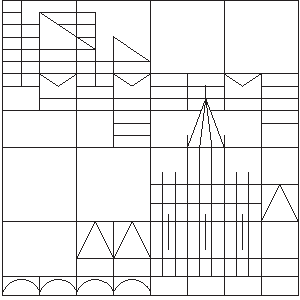
\includegraphics[scale=0.7]{figures/signet} % signet U KN
\end{center}
\vspace{4mm}
\rule{0.98\linewidth}{2pt}\\
\vspace{4mm} 
{\huge {\bf {\sffamily{Master Thesis}}}}\\
\vspace{10mm}
{\huge Building Decentralized Applications with Data Ownership }\\
\vspace{10mm}
{\em {\sffamily{in fulfillment of the requirements to achieve the degree of \\ 
\vspace{2mm} {\bf \sffamily{Master of Science (M.Sc.)}}}}}\\
\vspace{2mm}
\rule{0.98\linewidth}{2pt}\\
\vspace{10mm}{\Large \bf \sffamily{Harsh Kedia}}\\
\vspace{1mm}{Matriculation Number :: 01/752437}\\
\vspace{1mm}{E-Mail :: $\langle$harsh$\rangle$.$\langle$kedia$\rangle$@uni-konstanz.de}\\
\vspace{10mm}
{\footnotesize
\begin{tabular}{l  p{5mm}  r}
{\bf {\sffamily{Field of Study}}} ::  Information Engineering & & {\bf \sffamily{First Assessor}} ::  {\em Prof. Dr. M. Waldvogel}\\
{\bf {\sffamily{Focus}}} ::  {\em Applied Computer Science} & & {\bf \sffamily{Second Assessor}} ::  {\em Prof. Dr. S. Kosub}\\
{\bf {\sffamily{Topic}}} :: {\em Distributed Systems}& & {\bf \sffamily{Advisor}} ::  {\em Prof. Dr. M. Waldvogel}\\
\end{tabular}\\
}
\end{center}
}
\vfill
\end{titlepage}




 % include your titlepage here (standard title page with university signet)
\begin{titlepage}
\begin{minipage}{0.9\linewidth}
\end{minipage}
\vfill
\begin{center}
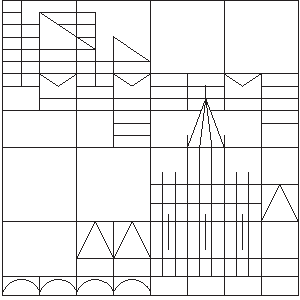
\includegraphics[scale=1]{figures/signet} % signet U KN
\end{center}
\vspace{10mm}
\vfill
{\sf
\begin{center}
{\Large University of  Konstanz} \\
\vspace{2mm}{\Large Department of Computer and Information Science} \\ 
\vspace{4mm}
\rule{0.98\linewidth}{2pt}\\
\vspace{4mm} 
{\huge {\bf {\sffamily{[Bachelor $|$ Master] Thesis}}}}\\
\vspace{10mm}
{\huge Your Thesis Title}\\
\vspace{10mm}
{\em {\sffamily{in fulfillment of the requirements to achieve the degree of \\ 
\vspace{2mm} {\bf \sffamily{[Bachelor of Science (B.Sc.) $|$ Master of Science (M.Sc.)]}}}}}\\
\vspace{2mm}
\rule{0.98\linewidth}{2pt}\\
\vspace{6mm}{\Large \bf \sffamily{Firstname Lastname}}\\
\vspace{0mm}{Matriculation Number :: 01/xxxxxx}\\
\vspace{0mm}{E-Mail :: $\langle$firstname$\rangle$.$\langle$lastname$\rangle$@uni-konstanz.de}\\
\vspace{6mm}
{\small
\begin{tabular}{l  p{5mm}  r}
{\bf {\sffamily{Field of Study}}} ::  Information Engineering & & {\bf \sffamily{First Assessor}} ::  {\em Prof. Dr. M. Waldvogel}\\
{\bf {\sffamily{Focus}}} ::  {\em Applied Computer Science} & & {\bf \sffamily{Second Assessor}} ::  {\em }\\
{\bf {\sffamily{Topic}}} :: {\em Distributed Systems}& & {\bf \sffamily{Advisor}} ::  {\em Prof. Dr. M. Waldvogel}\\
\end{tabular}\\
}
\end{center}
}
\vfill
\end{titlepage}




 % include your titlepage here (unconventional title page with university signet above 
\begin{titlepage}
\begin{minipage}{0.9\linewidth}
\end{minipage}
\vfill
{\sf
\begin{center}
{\Large University of  Konstanz} \\
\vspace{2mm}{\Large Department of Computer and Information Science} \\ 
\vspace{1mm}
\rule{0.98\linewidth}{2pt}\\
\vspace{3mm} 
{\huge {\bf {\sffamily{[Bachelor $|$ Master] Thesis}}}}\\
\vspace{8mm}
{\huge Your Thesis Title}\\
\vspace{8mm}
{\em {\sffamily{in fulfillment of the requirements to achieve the degree of \\ 
\vspace{2mm} {\bf \sffamily{[Bachelor of Science (B.Sc.) $|$ Master of Science (M.Sc.)]}}}}}\\
\vspace{1mm}
\rule{0.98\linewidth}{2pt}\\
\vspace{4mm}{\Large \bf \sffamily{Firstname Lastname}}\\
\vspace{0mm}{Matriculation Number :: 01/xxxxxx}\\
\vspace{0mm}{E-Mail :: $\langle$firstname$\rangle$.$\langle$lastname$\rangle$@uni-konstanz.de}\\
\vspace{4mm}
{\small
\begin{tabular}{l  p{5mm}  r}
{\bf {\sffamily{Field of Study}}} ::  Information Engineering & & {\bf \sffamily{First Assessor}} ::  {\em Prof. Dr. M. Waldvogel}\\
{\bf {\sffamily{Focus}}} ::  {\em Applied Computer Science} & & {\bf \sffamily{Second Assessor}} ::  {\em}\\
{\bf {\sffamily{Topic}}} :: {\em Distributed Systems}& & {\bf \sffamily{Advisor}} ::  {\em Prof. Dr. M. Waldvogel}\\
\end{tabular}\\
}
\end{center}
}
\end{titlepage}




 % include your titlepage here (unconventional title page with space for a teaser image)
%\pagestyle{fancy}

%%%%%%%%%%%%%%%%%%%%%%%%%%%%%%%%%%%%%%%%%%%%%%%%%%%%%%%%%%%%%%%%%%%%%%%%%%%%%%%%%%%%%%%%%%%%%%%%%%%%%%%%%%%%%%%%%
%%% PREAMBLE
%%%%%%%%%%%%%%%%%%%%%%%%%%%%%%%%%%%%%%%%%%%%%%%%%%%%%%%%%%%%%%%%%%%%%%%%%%%%%%%%%%%%%%%%%%%%%%%%%%%%%%%%%%%%%%%%%
\newpage
\pagestyle{fancy}
\voffset=10mm % optical enhancement!!!
\pagenumbering{roman} % set the page numbering style to roman numbers
\cleardoublepage
\thispagestyle{empty}
\vspace*{0.5\textheight}
\begin{center}
\textit{To}

My Mom,
\begin{sanskrit}
	निर्मला
\end{sanskrit}
\end{center}
\newpage % refer your preamble here

%%%%%%%%%%%%%%%%%%%%%%%%%%%%%%%%%%%%%%%%%%%%%%%%%%%%%%%%%%%%%%%%%%%%%%%%%%%%%%%%%%%%%%%%%%%%%%%%%%%%%%%%%%%%%%%%%
%%% ABSTRACT
%%%%%%%%%%%%%%%%%%%%%%%%%%%%%%%%%%%%%%%%%%%%%%%%%%%%%%%%%%%%%%%%%%%%%%%%%%%%%%%%%%%%%%%%%%%%%%%%%%%%%%%%%%%%%%%%%
\newpage
\setcounter{page}{1}
\begin{abstract}
Information requires data and an economy requires a unit of account. It's important that in the \textit{Information Economy} enabled by the internet, we own our data. Blockchain with its native token enables a unit of account. It also serves as the base layer for building a Decentralized Public Key Infrastructure (DPKI) enabling every individual to have a Self-Sovereign Identity. The concept of users owning their digital identity enables decentralized applications with Data Ownership.

This thesis explores the different concepts which make up a web application and describes how each can be decentralized using Blockchain and other peer-to-peer protocols. We analyze the state-of-the-art in decentralized applications platforms by building two \textit{proof-of-concept} applications for file sharing, one built on Ethereum and second built on Blockstack.

The main aim of the thesis is to provide its readers with a better understanding of what Blockchain technology enables and showcase certain properties of a secure decentralized applications platform.
\end{abstract} % refer your abstract here
\addcontentsline{toc}{section}{\abstractname}

%%%%%%%%%%%%%%%%%%%%%%%%%%%%%%%%%%%%%%%%%%%%%%%%%%%%%%%%%%%%%%%%%%%%%%%%%%%%%%%%%%%%%%%%%%%%%%%%%%%%%%%%%%%%%%%%%
%%% TABLE OF CONTENT, LIST OF FIGURES & LIST OF TABLES
%%%%%%%%%%%%%%%%%%%%%%%%%%%%%%%%%%%%%%%%%%%%%%%%%%%%%%%%%%%%%%%%%%%%%%%%%%%%%%%%%%%%%%%%%%%%%%%%%%%%%%%%%%%%%%%%%
\newpage
\setcounter{tocdepth}{2}
\tableofcontents{\thispagestyle{fancy}}
\newpage
\listoffigures
\addcontentsline{toc}{section}{\listfigurename}
\newpage
\listoftables
\addcontentsline{toc}{section}{\listtablename}

%%%%%%%%%%%%%%%%%%%%%%%%%%%%%%%%%%%%%%%%%%%%%%%%%%%%%%%%%%%%%%%%%%%%%%%%%%%%%%%%%%%%%%%%%%%%%%%%%%%%%%%%%%%%%%%%%
%%% SECTIONS
%%%%%%%%%%%%%%%%%%%%%%%%%%%%%%%%%%%%%%%%%%%%%%%%%%%%%%%%%%%%%%%%%%%%%%%%%%%%%%%%%%%%%%%%%%%%%%%%%%%%%%%%%%%%%%%%%
\cleardoublepage
\pagestyle{fancy}
\pagenumbering{arabic} % set the page numbering to arabic page numbers
%\setcounter{page}{1}
\chapter{Introduction}\label{chapter::introduction}
Humans have evolved over thousands of years building systems that deal with land ownership and property rights. With the advent of the Internet, our lives have become more and more digital, with data becoming the new currency in today's digital economy. However, we have no experience in managing data ownership. Big tech companies understood the importance of user data a long time ago. They offered their services free of charge in exchange for our data, which they then used to generate profits, control our perception about how we see the world, and also tamper with public affairs like the election. There is a need to define a model for data ownership and build systems that enable users to own their data.

With data ownership comes the question of digital identity. How can we identify ourselves over the Internet? With username and passwords, we can uniquely identify ourselves when using a service, but then we have to create an identity for each service we want to use. It has another drawback, i.e., our passwords are stored on a central server, which is prone to hacking. There exist systems like \textit{Google Sign-in} or \textit{Facebook Connect}, which allows us to carry our identity across multiple services, but then again, this identity is not owned by the user but by Google or Facebook. Therefore, there is a need for user-owned identity, which can be verified independently by anyone.

To visualize a model for Data Ownership, let us look at Land Ownership. In the land ownership model, at any given point in time, a property has a fixed Geo-location while the owner can be anywhere in the Geo-space. Conversely, In a data ownership model, at any given point in time, a user has a fixed identity while the data can be anywhere on the Internet.

Blockchain enables the peer-to-peer exchange of value across the Internet. Smart contracts, which are self-executing code running on a Blockchain, enable decentralized marketplaces. Finally, Blockchain's public key cryptography enables a Decentralized Public Key Infrastructure (DPKI), thereby empowering users to create self-sovereign identity. Combining self-sovereign identity with encrypted storage enables us to build systems where users own their identity as well as their data.

In this thesis, we present the concepts which make up a web application and analyze the state-of-the-art for building them in a decentralized way. We start by introducing the concepts and technologies which serve as the building blocks for decentralized protocols (Chapter~\ref{chapter::background}). We describe the three types of web applications and different concepts that make them up. We then describe the evolution of each concept and explain how they will evolve because of Blockchain technology and other peer-to-peer protocols. Combining the concepts at the application layer, we propose an architecture for building decentralized applications (Chapter~\ref{chapter::app-concepts-design}). Using this architecture, we built two proof-of-concepts applications using Ethereum and Blockstack, two popular decentralized applications ecosystem (Chapter~\ref{chapter:building-dapp}). We then compare and analyze the two applications and their underlying platform. We also compare similar protocols as used in the applications (Chapter~\ref{chapter::results}). We discuss the findings (Chapter~\ref{chapter::discussion}) and conclude with a short outlook into the future (Chapter~\ref{chapter::conclusion}).
 % refer your introduction here
%\cleardoublepage
%\section{Related Work}\label{sec::relatedwork} 
%\cleardoublepage
%\chapter{Application Design}\label{chapter::decentralizedapps}

\section{Introduction}
	An Application software or \textit{app} is a computer program designed to perform a specific set of tasks or actions for the end user. There are countless number of applications in use today and the majority of them are web applications following a centralized client-server model\cite{raval2016decentralized}.
	
	\begin{figure}[h]
		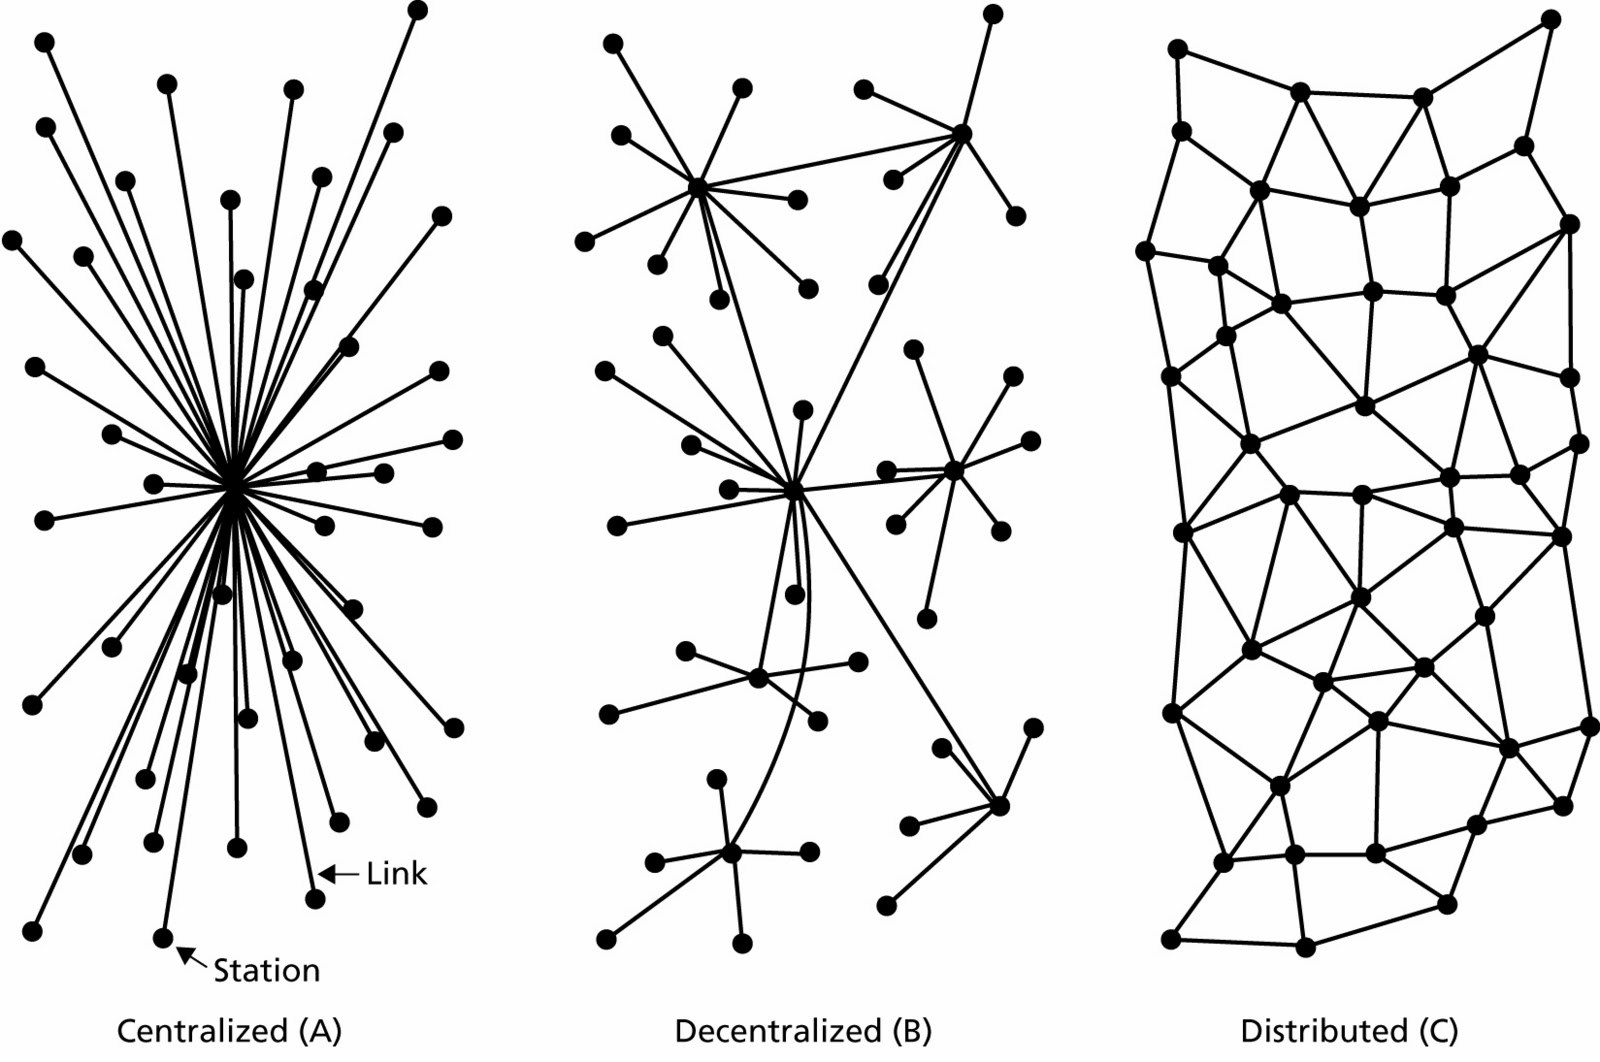
\includegraphics[width=\linewidth]{figures/network-models}
		\caption{\label{fig:applications} The three way of modeling web applications}
	\end{figure}
	
	Figure~\ref{fig:applications} shows a visual representation of three different ways of modeling web applications\cite{baran1964distributed}. Here, \textit{Centralized} and \textit{Decentralized} refers to level of control, while \textit{Distributed} refers to differences of location. Both centralized and decentralized systems can be distributed as well.
	
	\subsection{Centralized}
	It's currently the widespread way of building software applications. In this model a central server control the flow of information and governs the operation of individual units. Since the control is centralized, these types of systems suffer from single point of failure risk.
	
	\subsection{Distributed}
	In a Distributed model, the control still resides with a central server, however, the computation is spread across multiple nodes or servers.
	
	\subsection{Decentralized}
	In a Decentralized model, there is no central point of control as it's spread across all the servers running the application. Applications built using this model don't have a single point of failure and are inherently fault tolerant.

\section{Enabling Technologies}
	The document \textit{Information Management: A Proposal\cite{berners1989information}} written by \textit{Sir Tim Berners-Lee\footnote{\url{https://www.w3.org/People/Berners-Lee/}}} conceived the ideas for what would become the WorldWideWeb. It's main goal was to enable information exchange between computers in an accessible way at CERN\footnote{\url{https://home.cern/}}.
	
	HTML\footnote{\url{https://developer.mozilla.org/en-US/docs/Web/HTML}}, URI\footnote{\url{https://tools.ietf.org/html/rfc3986}} and HTTP\footnote{\url{https://tools.ietf.org/html/rfc2616}} were the fundamental technologies that defined the foundation of the Web. HTTP connected every computer on the planet with a common protocol. The HTTP protocol guidelines defined a set of trusted servers that translated a web address into a server address. Furthermore, HTTPS\footnote{\url{https://tools.ietf.org/html/rfc2818}} added another layer of trusted servers and certificate authorities. People would host personal servers for others to connect to, and everyone owned their data\cite{raval2016decentralized}. As the Web evolved, applications servers\footnote{\url{https://en.wikipedia.org/wiki/Application_server}} became the common way of interactive with the Web and the centralized model of data ownership as we know it today was born\cite{raval2016decentralized}. It was conceptually and programmatically easier to maintain an application server and profit from user's data that utilize it.
	
	Blockchain is the primary technology that enables the creation of applications with a decentralized model of data ownership. It puts the users of an application in control of their data thereby enabling a more open Web, as it was originally intended\footnote{\url{https://webfoundation.org/about/vision/history-of-the-web/}}.
	
	The blockchain helped solve the Byzantine Generals Problem\cite{lamport1982byzantine}. This problem describes a situation where all participating nodes in a distributed network must agree upon every message that is being transmitted between nodes, but where some of the nodes are corrupt and disseminating false information or are unreliable. This agreement is called as \textbf{consensus}. With Bitcoin\cite{nakamoto2008bitcoin}, decentralized consensus became possible. Agreement is achieved in the Bitcoin network by way of \textit{proof-of-work\footnote{\url{https://en.bitcoin.it/wiki/Proof_of_work}}} consensus mechanism which is resistant to Sybil Attack\cite{douceur2002sybil}. Proof-of work is both computationally and energy expensive; other consensus mechanism such as \textit{proof-of-stake\footnote{\url{https://en.bitcoin.it/wiki/Proof_of_Stake}}} relies on stake in the system instead of computational power.
	
\section{Concepts}
	There are five concepts in a web application that have traditionally been implemented in way that puts control with a centralized entity: data, identity, value, computing and bandwidth\cite{raval2016decentralized}. Each of these require trust in a 3rd party - a trust which can be betrayed. Recent advancements in distributed-system technology can put users in control of these things. Below sections describes each concept in detail and shows how one can build applications in a way such that centralized control is not required.

\section{Data}
	Data is the most important concept in any web application. First, let's look at how traditional web applications interact with data. Whenever, a user logs into an application, the application connects to a remote server and sends the authentication details. These details lets the server know which user is interacting with the application. Once authenticated, the user data is fetched from the remote storage and displayed to the user. All complex computations and data storage occurs on dedicated servers maintained in the cloud.
		
	\begin{figure}[h]
		\centering
		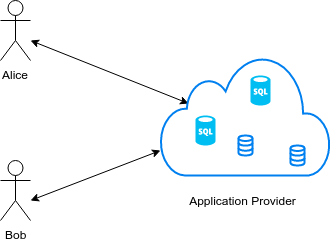
\includegraphics[width=200pt, height=150pt]{figures/traditional-app}
		\caption{\label{fig:traditional-app} How traditional web applications work}
	\end{figure}
		
	Figure~\ref{fig:traditional-app} shows how users interact with a traditional web application. Whenever, Alice wants to interact with Bob, she sends a message to the application server which then delivers the message to Bob. There is no direct path between Alice and Bob. This results in centralization where the provider acts as an intermediary between Alice and Bob's interaction; effectively governing how data is stored and shared among them.
		
	This model of application interaction requires that we trust the providers with out data and hope that they won't misuse or sell our data without our permission. Since revelations by Edward Snowden\cite{greenwald2014no}, we now know that trust can, has and will be broken as long as we entrust our data to a central entity\cite{raval2016decentralized}. Centralized stores of data also serve as a tool for surveillance, allowing big entities to monitor our internet behaviour without our knowledge. Cloud providers, despite having a distributed backend, are centrally owned.
		
	Additionally, as we move from a labor-based economy to an information-based economy, data will become the primary form of value. Therefore, its important that we not only possess our data, but own it as the world evolves. An ideal solution that enables this should provide a way of storing data in a decentralized way that is robust and as trustless as possible\cite{raval2016decentralized}.
	
	\subsection{Storing Data Directly in a Blockchain}
		This method does solves the decentralization of data as everyone who has copy of the Blockchain is storing the data but cannot alter it. The data can be encrypted such that it can only be accessed by someone having the private key. However, Blockchains were not meant for storing large amounts of data. It was designed for storing simple transactional logs, as its evident from looking at the Bitcoin Blockchain where individual records are in bytes\footnote{\url{https://en.bitcoin.it/wiki/Transaction}} and therefore cannot hold much data. Moreover, the Blockchain architecture implies that each node in the network must store a complete copy of the Blockchain. Therefore, storing a significant amount of data on a Blockchain is both expensive and impractical.
		
	\subsection{Storing Data in a Distributed Hash Table}
		DHTs ensure data resiliency by enabling easy distribution and indexing of data. Early peer-to-peer (P2P) filesharing applications like KaZaA\cite{good2003usability}, Napster\cite{ku2002creative} and Gnutella\cite{ripeanu2002mapping} used their own versions of DHTs with a varying degree of decentralization. Some had centralized trackers to monitor the movement of data, while some had central sources from which all data must pass, leaving them with single point of failure\cite{raval2016decentralized}.
		
		BitTorrent\cite{cohen2008bittorrent} was the first protocol to popularize DHT for sharing of large files. As of 2013, BitTorrent has 15–27 million concurrent users at any given time\cite{wang2013measuring}. The BitTorrent Mainline DHT serves as a decentralized data store with centralized trackers to monitor the network. It uses a tit-for-tat strategy between seeders and leechers to maximize the bandwidth of data distribution. This makes the BitTorrent protocol the de facto method for transfer of large datasets over the web. However, using BitTorrent as a data store is not feasible as there is no incentives for nodes to store a data leading to \textit{data impermanence}.
		
		Along with the decentralized storage capabilities of DHT and the speed of BitTorrent's protocol, we also want data permanence. Therefore, its necessary to incentivize the nodes storing the data in some way. Moreover, we also need to ensure that the links to the data don't die, an idea which was first proposed in Project Xanadu\cite{rayward1994visions}.
		
		\subsubsection{InterPlanetary File System (IPFS)} 
			IPFS\cite{benet2014ipfs} is a peer-to-peer file transfer protocol that implements these features, enabling a more permanent, decentralized Web, where links don't die and no single entity controls the data. It achieves this by combining previous peer-to-peer technologies such as DHT, BitTorrent and Git\cite{loeliger2012version}. Data in the IPFS network is modeled as a \textit{merkleDAG\footnote{Similar to a Merkle tree data structure, however, they do not need to be balanced and it's non-leaf nodes can contain some data.}}, a simple data structure that can be conceptualized as a series of nodes connected to each other\cite{raval2016decentralized}. This makes IPFS a \textit{content-addressed\footnote{A content-addressed storage is way to store information such that it can retrieved based on its content and not its location.}} system allowing efficient data lookup and retrieval as it doesn't rely on a single server to access the data.
		
			\begin{figure}[h]
				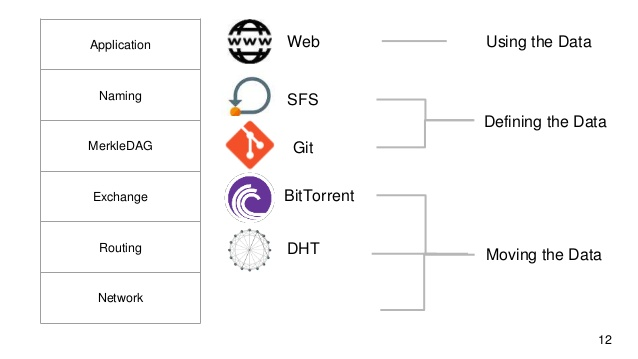
\includegraphics[width=\linewidth]{figures/ipfs-stack}
				\caption{\label{fig:ipfs-stack} IPFS Stack}
			\end{figure}
		
			Filecoin\cite{benet2018filecoin}, a \textit{decentralized storage network}, combines IPFS (shown in Figure~\ref{fig:ipfs-stack}\footnote{Adopted from: \url{https://image.slidesharecdn.com/ipfs-171229085327/95/ipfs-12-638.jpg?cb=1514537643}}) with an incentive structure that turns cloud storage into an algorithmic market effectively overcoming the limitations of BitTorrent. This market runs on a blockchain with a native protocol token, which miners earn by providing storage to clients.
		
	\subsection{Storing Data in a Cloud in Encrypted Containers}
		IPFS enables a way for decentralized storage such that it overcomes the single point of failure risk, however, the user does not control where the data is being stored. Because of this, once a data is added to the network, and is picked up by other nodes for re-hosting, it cannot be taken back as there is no way to verify information deletion\footnote{\url{https://github.com/ipfs/faq/issues/9}}.
		
		\subsubsection{Gaia: User-Controlled Storage}
		Gaia\cite{ali2016blockstack} is a decentralized storage system that enables user-controlled private data lockers. It works by hosting data in one or more existing storage systems of user's choice. Data on Gaia is encrypted and signed by user-controlled cryptographic keys before being uploaded to a provider. Storing data using existing cloud infrastructure ensures high data availability without compromising on application performance. Further, since each data is signed by keys which a user controls, it ensures that they don't need to trust the underlying cloud providers.
		
		\begin{figure}[h]
			\centering
			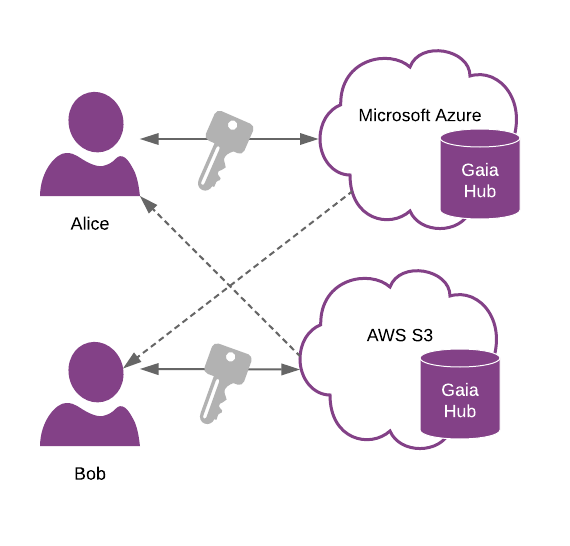
\includegraphics[width=200pt, height=200pt]{figures/gaia-storage}
			\caption{\label{fig:gaia-storage} How users interact with Gaia storage\protect\footnotemark}
		\end{figure}
		\footnotetext{\url{https://docs.blockstack.org/storage/overview.html}}
		
		Writing data to a Gaia hub involves a \texttt{POST} request along with a signed \textit{authentication} token. This token is signed by the private key which controls the particular bucket being written to. Separate buckets are used for each application, this ensures that a given private key grants access only to a specific bucket on the Gaia Server.
		
		\begin{figure}[h]
			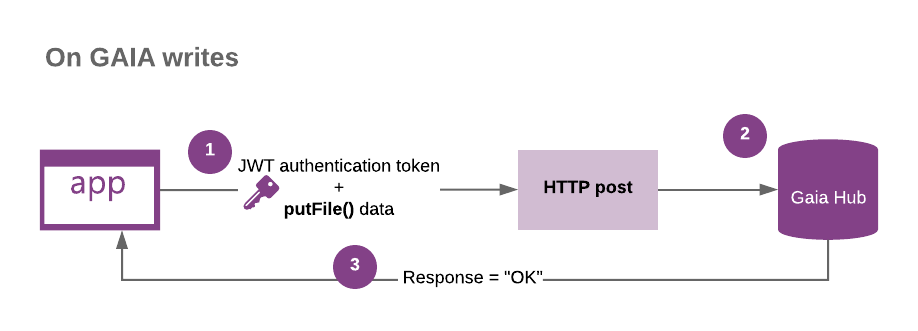
\includegraphics[width=\linewidth]{figures/gaia-writes}
			\caption{\label{fig:gaia-writes} The token ensures that a write is authorized\protect\footnotemark}
		\end{figure}
		\footnotetext{\url{https://docs.blockstack.org/storage/authentication.html}}
		
		Reading data from a user's Gaia hub involves a \textit{zonefile} lookup. This zonefile is a signed JSON object containing the URLs pointing to the user's Gaia data locker. Once verified that the zonefile is signed by user's key, a standard \texttt{HTTP} request is made to fetch the requested data.
		
		Figure~\ref{fig:gaia-overview} shows an overview of Gaia. Looking up data for a name works as follows:
		
		\begin{enumerate}
			\item Lookup the \textit{name} in the Virtualchain to get the (\textit{name, hash}) pair.
			\item Lookup the \textit{hash(name)} in Peer Network to get respective zonefile.
			\item Get the user's Gaia URL from the zonefile and lookup the URL to connect to storage backend.
			\item Fetch the requested data and verify the respective signature or hash.
		\end{enumerate}
		
		\begin{figure}[h]
			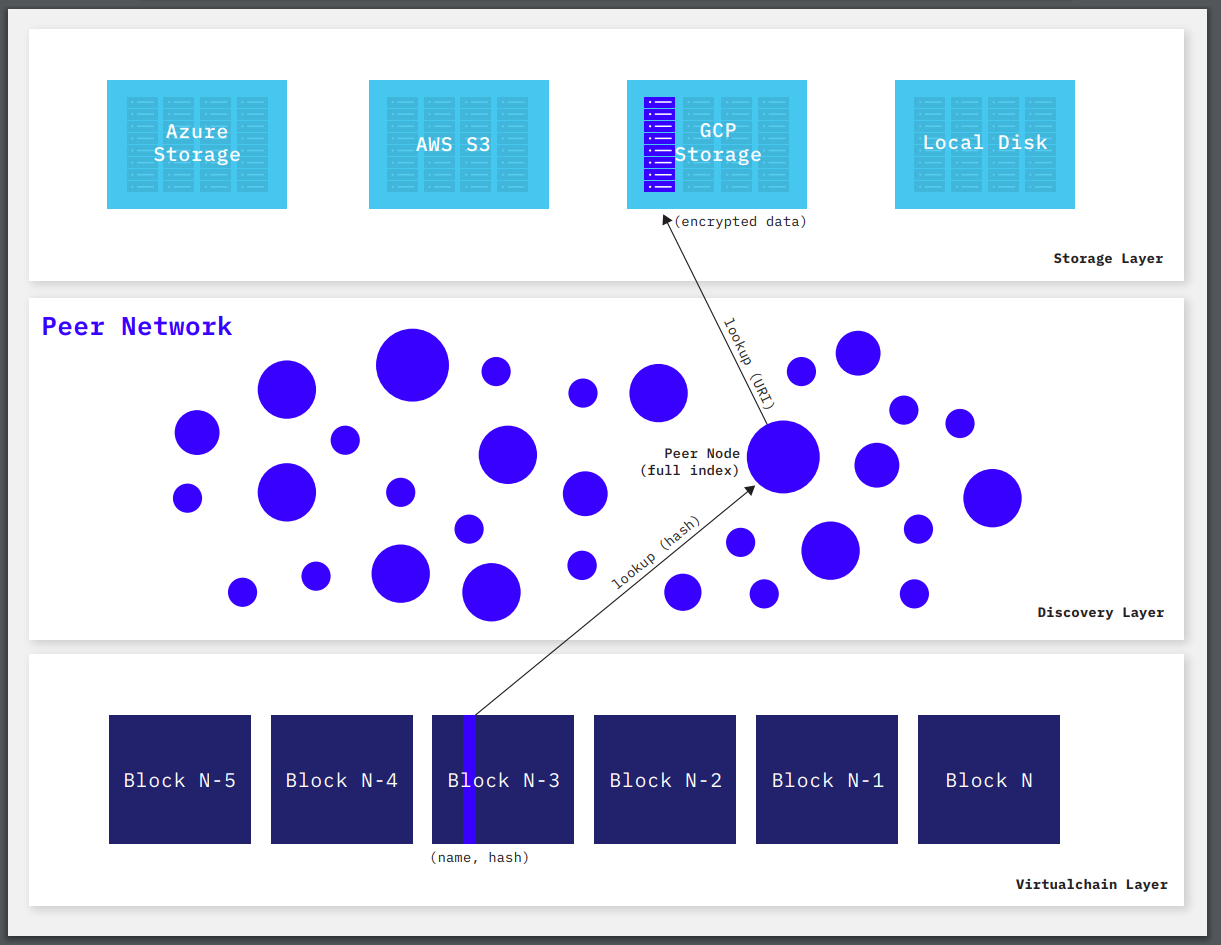
\includegraphics[width=\linewidth]{figures/gaia-overview}
			\caption{\label{fig:gaia-overview} Overview of Gaia and steps for looking up data.\protect\footnotemark}
		\end{figure}
		\footnotetext{\url{https://blockstack.org/whitepaper.pdf}}
		
	
\section{Identity}
	User identities are essential to using internet applications. In order to confirm their identity, users must provide some information. This information depends on the application's authentication process. If an application maintains a user database, it requires a username and a password and sometimes a second factor. If an application relies on a third-party, like Google\footnote{\url{https://developers.google.com/identity/}} or Facebook\footnote{\url{https://developers.facebook.com/docs/facebook-login/}} for identity management, it uses the OAuth 2.0 authentication\cite{hardt2012oauth} protocol, which identifies a user by generating an assertion from the identity service.
	
	Third party identity providers implementing the OAuth\footnote{\url{https://oauth.net/}} protocol often have their own version of implementation which leads to identity fragmentation across the web. OpenID\cite{recordon2006openid} is a decentralized identity protocol that allows users to create one identity which can be carried across multiple providers. However, the user still needs to trust one of the service providers with their identity information\cite{raval2016decentralized}.
	
	Another way of authenticating users with an application is by using digital certificates\cite{tycksen2001digital}. These certificates provide a proof of ownership of a public key. Authentication and management of public keys is facilitated using a Public Key Infrastructure (PKI)\cite{adams2003understanding} system. Currently, the most common approaches to PKIs are: Certificate Authorities (CAs) and PGP Web of Trust\cite{abdul1997pgp}. 
	
	A Certificate Authority (CA) acts a trusted third party responsible for management and distribution of digital certificates for a network of users\cite{fromknecht2014decentralized}. These trusted third parties introduces central control in a PKI system making them prone to single point of failure risk\cite{dooley2001designing}.
	
	In PGP Web of trust, authentication is entirely decentralized; users are able to designate others as trustworthy by signing their public keys. This process generates a digital certificate containing the user's public key and signatures from entities that have deemed him trustworthy. This system does benefit from its distributed nature as there is no central control. However, PGP does not offer identity retention. There is no guarantee of consistency and nothing prevents multiple users from creating public keys for the same identity\cite{fromknecht2014decentralized}.
	
	\subsection{Decentralized Public Key Infrastructure (DPKI)}
		\begin{figure}[h]
			\centering
			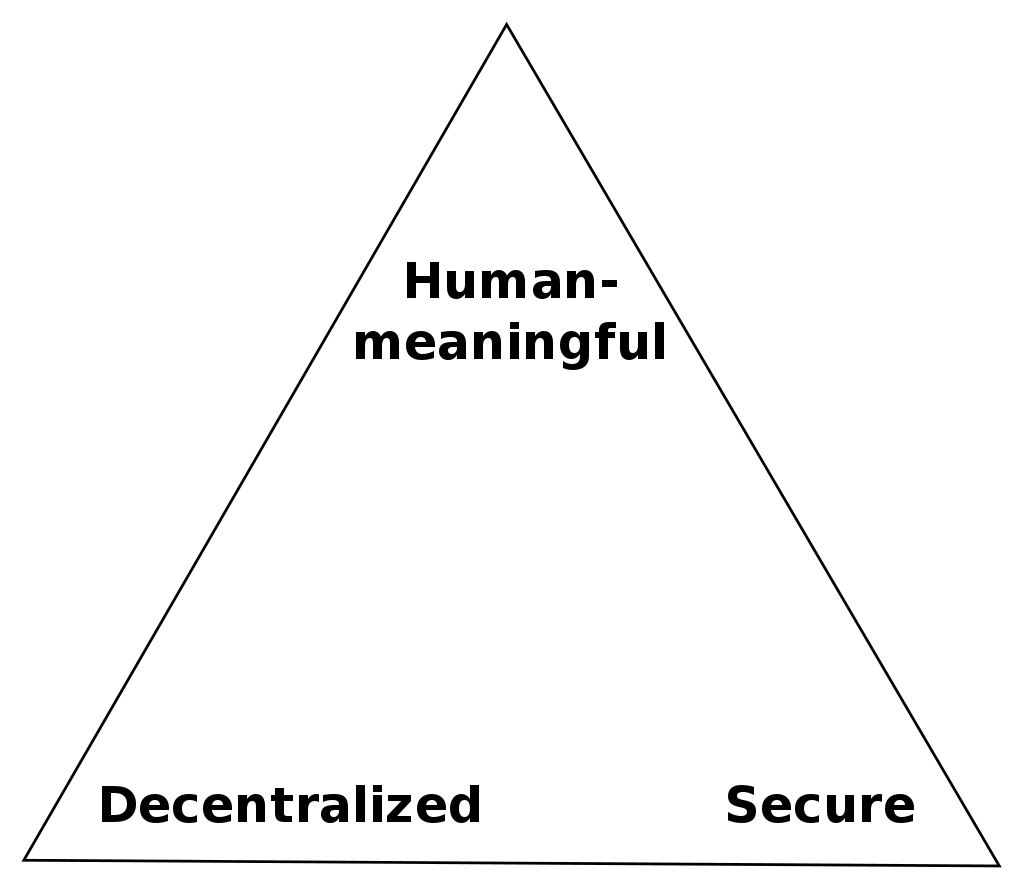
\includegraphics[width=200pt, height=150pt]{figures/zooko-triangle}
			\caption{\label{fig:zooko-triangle} Zooko's Triangle\protect\footnotemark}
		\end{figure}
		\footnotetext{\url{https://commons.wikimedia.org/wiki/File:Zooko\%27s_Triangle.svg}}
		
		The foundational precept of a DPKI is that \textit{identities belong to the entities they represent}. This requires designing a \textit{decentralized} infrastructure where every identity is controlled by its \textit{principal owner} and not by some trusted third party\cite{allen2015decentralized}.
		
		DPKI is essentially a system to gives unique names to participants in a network protocol. These names should have three desirable traits(Zooko's triangle) namely: \textit{Human-meaningful}, \textit{Decentralized} and \textit{Secure}. OpenID solved security and human-meaningfulness.
		
		Namecoin\footnote{\url{https://www.namecoin.org/}} was the first working solution that satisfied all three traits of Zooko's triangle by adding decentralization. It was the first fork of Bitcoin\cite{nakamoto2008bitcoin} protocol designed to act as a decentralized domain name server (DNS) for \textit{.bit} addresses. Namecoin's blockchain essentially could be used as an intermediary between a user and the service requesting user's identity\cite{raval2016decentralized}. It allowed a user to \textit{register} a name by creating a blockchain transaction. This transaction included the desired name which get embedded under the \textit{/id} namespace.
	
	\subsection{Decentralized Identifiers (DIDs)}
	A DID\footnote{\url{https://w3c-ccg.github.io/did-spec/}} is a new type of identifier that is globally unique, resolvable with high availability and cryptographically verifiable. DIDs typically contains cryptographic key pair which enables the controller of a DID to prove control over it.
	
	The concept of global unique decentralized identifiers is not new; Universally Unique Identifiers\footnote{\url{https://en.wikipedia.org/wiki/Universally_unique_identifier}}(UUIDs), also called Globally Unique Identifiers (GUIDs) were first such identifiers developed in 1980s and formally specified in RFC4122\footnote{\url{https://tools.ietf.org/html/rfc4122}}. Another class of identifiers knows as persistent identifiers was standardized as Uniform Resource Names (URNs) by RFC8141\footnote{\url{https://tools.ietf.org/html/rfc8141}}.
	
	However, UUIDs are not globally resolvable and URNs, if resolvable, require a central registry. Further, neither UUIDs or URNs have the ability to cryptographically verify ownership of the identifier. DIDs, on the other hand, fulfills all four requirements: persistence, global resolvability, cryptographically verifiability, and decentralization required for a self-sovereign identity\cite{smith2016identity}.
	
	\begin{figure}[h]
		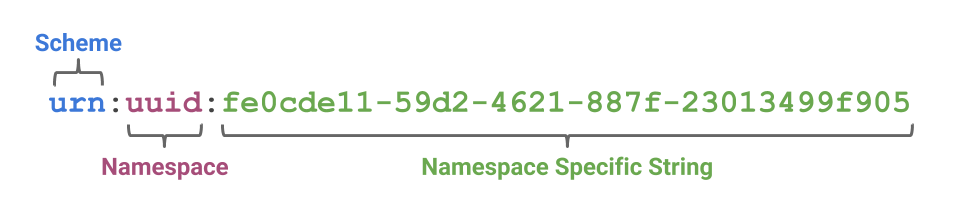
\includegraphics[width=\linewidth]{figures/urn-format}
		\caption{\label{fig:urn-format} The URN Specification}
	\end{figure}

	\begin{figure}[h]
		
\includegraphics[width=\linewidth]{figures/did-format}
		\caption{\label{fig:did-format} The DID Specification}
	\end{figure}
	
	The DID (Figure~\ref{fig:did-format}\footnote{\url{https://w3c-ccg.github.io/did-primer/did-primer-diagrams/did-format.png}}) specification follows the same pattern as the URN (Figure~\ref{fig:urn-format}\footnote{\url{https://w3c-ccg.github.io/did-primer/did-primer-diagrams/urn-format.png}}) specification. The key difference is that with DIDs, the namespace component identifies a \textit{DID method} which defines how DIDs work with a specific blockchain. The \textit{DID method} specifications must define the format and generation of the method-specific identifier. The DID methods can also be developed for identifiers registered in federated or centralized identity management systems, thus creating a interoperability bridge between the worlds of centralized, federated and decentralized identifiers.
	
\section{Value}
	
\section{Computing}
	
\section{Bandwidth}
\cleardoublepage
\section{Smart Contracts}\label{sec::smartcontracts}

\subsection{Introduction}

\subsection{Smart Contract Platforms}

\subsection{Smart Contract Vulnerabilities}

\subsection{Secure Smart Contracts}
\cleardoublepage
\section{Scalable Decentralized Applications}\label{sec::scalabledapps}
\cleardoublepage
\chapter{PoC 1: Ethereum dApp}\label{chapter:poc1}

\section{Introduction}
Existing applications for sharing files are central solutions and therefore suffer from single point of failure risk. Moreover, using central services for securing data means that we have to trust a 3rd party with our data thus exposing it to manipulation risks. Hence, a decentralized
application is required to overcome the problems posed by a central application. With the recent developments in Blockchain technology and P2P storage, it is possible to securely store and share data without using any central server.

This chapter describes the workings of the application \textit{dShare}\cite{harsh_kedia_2019_3359852} built using P2P technologies enabling a secure way of storing and sharing data between two individuals or entities. The latest version of the application is deployed at \url{https://file-share-dapp.herokuapp.com/}

\section{Technologies Used}

\subsection{Ethereum}
Ethereum\cite{buterin2014ethereum} is a blockchain platform for building decentralized applications. It allows the creation of \textit{Smart Contracts}. Solidity\footnote{\url{https://github.com/ethereum/solidity}} is the primary language for writing smart contracts on Ethereum.

\subsection{InterPlanetary File System (IPFS)}
IPFS\cite{benet2014ipfs} is a peer-to-peer file transfer protocol which enables a shared file system between all its connected peers. It achieves this by combining previous peer-to-peer systems such as Distributed Hash Tables (DHT), BitTorrent\cite{cohen2008bittorrent}, and Git\cite{loeliger2012version}. The data in the IPFS network are modeled as a Merkle DAG\footnote{Merkle directed acyclic graph - similiar to a Merkle tree data structure however they do not need to be balanced and it’s non-leaf nodes can contain some data.} thus providing a throughput storage system with content-addressed hyperlinks.

\begin{figure}[h]
	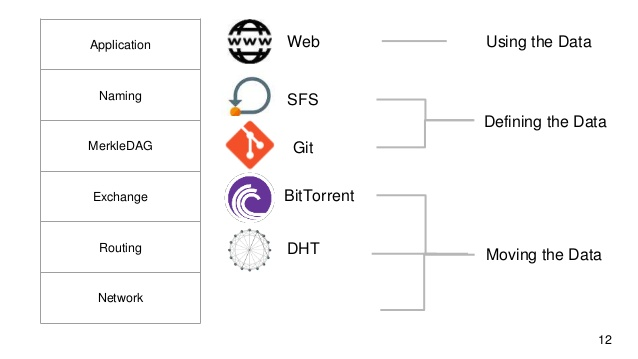
\includegraphics[width=\linewidth]{figures/ipfs-stack}
	\caption{\label{fig:ipfs-stack} IPFS Stack}
\end{figure}

Figure~\ref{fig:ipfs-stack}\footnote{Adopted from: \url{https://image.slidesharecdn.com/ipfs-171229085327/95/ipfs-12-638.jpg?cb=1514537643}} shows the IPFS Stack. It consists of sub-protocols, each providing a different functionality.

\begin{itemize}
	\item Identities - node identification and verification.
	\item Network - connection management among peers.
	\item Routing - peer lookup using DHT.
	\item Exchange - data exchange strategies among peers.
	\item Objects - a content-addressed Merkle DAG.
	\item Files - versioned file system.
	\item Naming - A self-certifying mutable name system.
\end{itemize}

\subsection{OriginStamp}
OriginStamp\cite{hepp2018originstamp} is a blockchain based system for decentralized timestamping. It uses the Bitcoin blockchain for the creation of trusted and immutable timestamps for any piece of data. Timestamps created by OriginStamp can be verified independently by anyone.

\begin{figure}[h]
	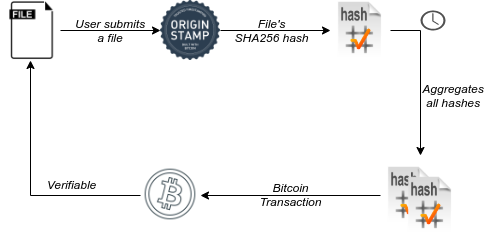
\includegraphics[width=\linewidth]{figures/origin-stamp}
	\caption{\label{fig:originstamp} Timestamping using OriginStamp}
\end{figure}

Figure~\ref{fig:originstamp} visualizes the timestamping process as implemented in OriginStamp. When a user submits a file, the hash of the data is recorded. It combines all the hashes submitted over a period of time and generates an aggregated hash. After some additional hashing and encoding operations, a Bitcoin address is created to which the smallest possible transactional amount of Bitcoins is transferred. Performing this transaction embeds the hash and the timestamp permanently to the Bitcoin blockchain. Each transaction is part of a block and is added to the Bitcoin blockchain by a process called mining. Since each block is linked cryptographically to the previous block, adding a new block confirms the validity of the last block. Changing the timestamp of a transaction becomes impossible once five or six subsequent blocks are mined, which requires an hour on average\cite{nakamoto2008bitcoin}.

\section{Implementation}
For storing of files we used IPFS. Before uploading to the IPFS network, files are encrypted using AES-GCM encryption mechanism. Sharing of encryption keys is facilitated using smart contracts built on Ethereum; thus files can be shared by anyone with an Ethereum address. Finally, OriginStamp is used for immutable timestamping.

The front-end of the application is built using React.js, a JavaScript library for building user interfaces. Solidity was used for writing smart contracts and deployed on the Ethereum test network, Rinkeby. Next.js was used for server-side rendering (SSR), and Firebase was used as a database for storing public Ethereum key of the users.

\section{Working}
\cleardoublepage
\chapter{Example Application 2}\label{chapter:poc2}

\section{Introduction}

\section{Technologies Used}

\section{Implementation}

\section{Working}
%\cleardoublepage
%\chapter{Discussion}\label{chapter::discussion}

	Chapter~\ref{chapter::results} analyzed and compared the two \textit{proof-of-concept} applications and their underlying technology. This chapter focuses on interpreting the results and showing the state-of-the-art in decentralized technologies for building applications with data ownership. 
	
	\section{On Decentralized Application Platform}
	Analyzing the underlying platforms on which the two applications are built, its clear that Blockstack, due to its layered architecture is much more flexible and robust than Ethereum. Blockstack's separation of computations and storage from the blockchain layer makes it easier to scale and upgrade. It's integrated DPKI system offers its users with a self-sovereign identity. Building applications around the concept of a decentralized identity enable us to build a web where everyone owns their data.
	
	Ethereum, too is moving towards a layered architecture with their Eth 2.0 upgrade. The upgrade is spread across three phases. The complete specifications for the upgrade can be found at \url{https://github.com/ethereum/eth2.0-specs}.
	
	\section{On Decentralized Storage}
	Applications with data ownership involves encrypted data where storage systems are incentivized to store data. IPFS (see Section~\ref{sec:ipfs}) offers a content-addressed storage systems using p2p technologies like DHT, Git and BitTorrent. Gaia (see Section~\ref{sec:blockstack-gaia}) offers mutable data storage using existing cloud infrastructure. It's clear that both IPFS and Gaia enables a decentralized storage system serving different use cases. IPFS is more suitable for applications where nature of data is immutable and where decentralization precedes performance. Gaia, on the hand, is more suitable for applications where is data is mutable and data availability is crucial.
	
	\section{On Blockchains}
	Blockchain is the key enabler for building decentralized applications. It serves as the layer for value transfer in the Internet protocol stack. As inferred from results, blockchains based on \textit{proof-of-stake} are much more scalable and computationally inexpensive to use than blockchains based on \textit{proof-of-work}. Since, Blockchain enables a peer-to-peer information economy, it important that its built with strong security guarantees. Also, as public blockchains don't have a single entity controlling the system, its important for a blockchain to have a treasury and a governance system.
	
%\cleardoublepage
%\section{Conclusion}\label{sec::conclusion}

%%%%%%%%%%%%%%%%%%%%%%%%%%%%%%%%%%%%%%%%%%%%%%%%%%%%%%%%%%%%%%%%%%%%%%%%%%%%%%%%%%%%%%%%%%%%%%%%%%%%%%%%%%%%%%%%%
%%% APPENDIX
%%%%%%%%%%%%%%%%%%%%%%%%%%%%%%%%%%%%%%%%%%%%%%%%%%%%%%%%%%%%%%%%%%%%%%%%%%%%%%%%%%%%%%%%%%%%%%%%%%%%%%%%%%%%%%%%%
\cleardoublepage
\appendix
\chapter{Acknowledgements}
	I would like to thank my advisor Prof. Dr. Marcel Waldvogel, for his guidance and constructive discussions throughout my research. It helped me understand the principles of Distributed systems and how those principles apply to Blockchains. I am thankful to my supervisor Robert Müller who always found my ideas interesting and helped me limit my thesis scope.
	
	I am grateful to all my friends who helped me understand Blockchain from the perspectives of Economics, Philosophy, Psychology, and Mathematics. I am also grateful to authors like Yuval Noah Harari for `Sapiens: A Brief History of Humankind' and Raoul Martinez for `Creating Freedom: Power, Control and the Fight for Our Future,' which helped me understand Human Evolution and Human Behavior.  Without this holistic understanding, this thesis wouldn't have been possible.
	
	I would also like to thank Jun.-Prof. Dr. Stephan Streuber for giving me the opportunity to work on Virtual Reality projects involving collective behavior while working on my thesis. This helped me explore my other interests in Computer Science. % refer your acknowledgments here
%\input{statement}

%%%%%%%%%%%%%%%%%%%%%%%%%%%%%%%%%%%%%%%%%%%%%%%%%%%%%%%%%%%%%%%%%%%%%%%%%%%%%%%%%%%%%%%%%%%%%%%%%%%%%%%%%%%%%%%%%
%%% BIBLIOGRAPHY
%%%%%%%%%%%%%%%%%%%%%%%%%%%%%%%%%%%%%%%%%%%%%%%%%%%%%%%%%%%%%%%%%%%%%%%%%%%%%%%%%%%%%%%%%%%%%%%%%%%%%%%%%%%%%%%%%
\clearpage
\bibliographystyle{IEEEtran}
\bibliography{disy_thesis}
\addcontentsline{toc}{section}{References}

%%%%%%%%%%%%%%%%%%%%%%%%%%%%%%%%%%%%%%%%%%%%%%%%%%%%%%%%%%%%%%%%%%%%%%%%%%%%%%%%%%%%%%%%%%%%%%%%%%%%%%%%%%%%%%%%%
%%% EOD -- That's it folks!!!
%%%%%%%%%%%%%%%%%%%%%%%%%%%%%%%%%%%%%%%%%%%%%%%%%%%%%%%%%%%%%%%%%%%%%%%%%%%%%%%%%%%%%%%%%%%%%%%%%%%%%%%%%%%%%%%%%
\end{document}
